% Options for packages loaded elsewhere
\PassOptionsToPackage{unicode}{hyperref}
\PassOptionsToPackage{hyphens}{url}
\PassOptionsToPackage{dvipsnames,svgnames,x11names}{xcolor}
%
\documentclass[
  letterpaper,
  DIV=11,
  numbers=noendperiod]{scrartcl}

\usepackage{amsmath,amssymb}
\usepackage{iftex}
\ifPDFTeX
  \usepackage[T1]{fontenc}
  \usepackage[utf8]{inputenc}
  \usepackage{textcomp} % provide euro and other symbols
\else % if luatex or xetex
  \usepackage{unicode-math}
  \defaultfontfeatures{Scale=MatchLowercase}
  \defaultfontfeatures[\rmfamily]{Ligatures=TeX,Scale=1}
\fi
\usepackage{lmodern}
\ifPDFTeX\else  
    % xetex/luatex font selection
\fi
% Use upquote if available, for straight quotes in verbatim environments
\IfFileExists{upquote.sty}{\usepackage{upquote}}{}
\IfFileExists{microtype.sty}{% use microtype if available
  \usepackage[]{microtype}
  \UseMicrotypeSet[protrusion]{basicmath} % disable protrusion for tt fonts
}{}
\makeatletter
\@ifundefined{KOMAClassName}{% if non-KOMA class
  \IfFileExists{parskip.sty}{%
    \usepackage{parskip}
  }{% else
    \setlength{\parindent}{0pt}
    \setlength{\parskip}{6pt plus 2pt minus 1pt}}
}{% if KOMA class
  \KOMAoptions{parskip=half}}
\makeatother
\usepackage{xcolor}
\setlength{\emergencystretch}{3em} % prevent overfull lines
\setcounter{secnumdepth}{-\maxdimen} % remove section numbering
% Make \paragraph and \subparagraph free-standing
\makeatletter
\ifx\paragraph\undefined\else
  \let\oldparagraph\paragraph
  \renewcommand{\paragraph}{
    \@ifstar
      \xxxParagraphStar
      \xxxParagraphNoStar
  }
  \newcommand{\xxxParagraphStar}[1]{\oldparagraph*{#1}\mbox{}}
  \newcommand{\xxxParagraphNoStar}[1]{\oldparagraph{#1}\mbox{}}
\fi
\ifx\subparagraph\undefined\else
  \let\oldsubparagraph\subparagraph
  \renewcommand{\subparagraph}{
    \@ifstar
      \xxxSubParagraphStar
      \xxxSubParagraphNoStar
  }
  \newcommand{\xxxSubParagraphStar}[1]{\oldsubparagraph*{#1}\mbox{}}
  \newcommand{\xxxSubParagraphNoStar}[1]{\oldsubparagraph{#1}\mbox{}}
\fi
\makeatother

\usepackage{color}
\usepackage{fancyvrb}
\newcommand{\VerbBar}{|}
\newcommand{\VERB}{\Verb[commandchars=\\\{\}]}
\DefineVerbatimEnvironment{Highlighting}{Verbatim}{commandchars=\\\{\}}
% Add ',fontsize=\small' for more characters per line
\usepackage{framed}
\definecolor{shadecolor}{RGB}{241,243,245}
\newenvironment{Shaded}{\begin{snugshade}}{\end{snugshade}}
\newcommand{\AlertTok}[1]{\textcolor[rgb]{0.68,0.00,0.00}{#1}}
\newcommand{\AnnotationTok}[1]{\textcolor[rgb]{0.37,0.37,0.37}{#1}}
\newcommand{\AttributeTok}[1]{\textcolor[rgb]{0.40,0.45,0.13}{#1}}
\newcommand{\BaseNTok}[1]{\textcolor[rgb]{0.68,0.00,0.00}{#1}}
\newcommand{\BuiltInTok}[1]{\textcolor[rgb]{0.00,0.23,0.31}{#1}}
\newcommand{\CharTok}[1]{\textcolor[rgb]{0.13,0.47,0.30}{#1}}
\newcommand{\CommentTok}[1]{\textcolor[rgb]{0.37,0.37,0.37}{#1}}
\newcommand{\CommentVarTok}[1]{\textcolor[rgb]{0.37,0.37,0.37}{\textit{#1}}}
\newcommand{\ConstantTok}[1]{\textcolor[rgb]{0.56,0.35,0.01}{#1}}
\newcommand{\ControlFlowTok}[1]{\textcolor[rgb]{0.00,0.23,0.31}{\textbf{#1}}}
\newcommand{\DataTypeTok}[1]{\textcolor[rgb]{0.68,0.00,0.00}{#1}}
\newcommand{\DecValTok}[1]{\textcolor[rgb]{0.68,0.00,0.00}{#1}}
\newcommand{\DocumentationTok}[1]{\textcolor[rgb]{0.37,0.37,0.37}{\textit{#1}}}
\newcommand{\ErrorTok}[1]{\textcolor[rgb]{0.68,0.00,0.00}{#1}}
\newcommand{\ExtensionTok}[1]{\textcolor[rgb]{0.00,0.23,0.31}{#1}}
\newcommand{\FloatTok}[1]{\textcolor[rgb]{0.68,0.00,0.00}{#1}}
\newcommand{\FunctionTok}[1]{\textcolor[rgb]{0.28,0.35,0.67}{#1}}
\newcommand{\ImportTok}[1]{\textcolor[rgb]{0.00,0.46,0.62}{#1}}
\newcommand{\InformationTok}[1]{\textcolor[rgb]{0.37,0.37,0.37}{#1}}
\newcommand{\KeywordTok}[1]{\textcolor[rgb]{0.00,0.23,0.31}{\textbf{#1}}}
\newcommand{\NormalTok}[1]{\textcolor[rgb]{0.00,0.23,0.31}{#1}}
\newcommand{\OperatorTok}[1]{\textcolor[rgb]{0.37,0.37,0.37}{#1}}
\newcommand{\OtherTok}[1]{\textcolor[rgb]{0.00,0.23,0.31}{#1}}
\newcommand{\PreprocessorTok}[1]{\textcolor[rgb]{0.68,0.00,0.00}{#1}}
\newcommand{\RegionMarkerTok}[1]{\textcolor[rgb]{0.00,0.23,0.31}{#1}}
\newcommand{\SpecialCharTok}[1]{\textcolor[rgb]{0.37,0.37,0.37}{#1}}
\newcommand{\SpecialStringTok}[1]{\textcolor[rgb]{0.13,0.47,0.30}{#1}}
\newcommand{\StringTok}[1]{\textcolor[rgb]{0.13,0.47,0.30}{#1}}
\newcommand{\VariableTok}[1]{\textcolor[rgb]{0.07,0.07,0.07}{#1}}
\newcommand{\VerbatimStringTok}[1]{\textcolor[rgb]{0.13,0.47,0.30}{#1}}
\newcommand{\WarningTok}[1]{\textcolor[rgb]{0.37,0.37,0.37}{\textit{#1}}}

\providecommand{\tightlist}{%
  \setlength{\itemsep}{0pt}\setlength{\parskip}{0pt}}\usepackage{longtable,booktabs,array}
\usepackage{calc} % for calculating minipage widths
% Correct order of tables after \paragraph or \subparagraph
\usepackage{etoolbox}
\makeatletter
\patchcmd\longtable{\par}{\if@noskipsec\mbox{}\fi\par}{}{}
\makeatother
% Allow footnotes in longtable head/foot
\IfFileExists{footnotehyper.sty}{\usepackage{footnotehyper}}{\usepackage{footnote}}
\makesavenoteenv{longtable}
\usepackage{graphicx}
\makeatletter
\def\maxwidth{\ifdim\Gin@nat@width>\linewidth\linewidth\else\Gin@nat@width\fi}
\def\maxheight{\ifdim\Gin@nat@height>\textheight\textheight\else\Gin@nat@height\fi}
\makeatother
% Scale images if necessary, so that they will not overflow the page
% margins by default, and it is still possible to overwrite the defaults
% using explicit options in \includegraphics[width, height, ...]{}
\setkeys{Gin}{width=\maxwidth,height=\maxheight,keepaspectratio}
% Set default figure placement to htbp
\makeatletter
\def\fps@figure{htbp}
\makeatother

\usepackage{fvextra}
\DefineVerbatimEnvironment{Highlighting}{Verbatim}{breaklines,commandchars=\\\{\}}
\KOMAoption{captions}{tableheading}
\makeatletter
\@ifpackageloaded{caption}{}{\usepackage{caption}}
\AtBeginDocument{%
\ifdefined\contentsname
  \renewcommand*\contentsname{Table of contents}
\else
  \newcommand\contentsname{Table of contents}
\fi
\ifdefined\listfigurename
  \renewcommand*\listfigurename{List of Figures}
\else
  \newcommand\listfigurename{List of Figures}
\fi
\ifdefined\listtablename
  \renewcommand*\listtablename{List of Tables}
\else
  \newcommand\listtablename{List of Tables}
\fi
\ifdefined\figurename
  \renewcommand*\figurename{Figure}
\else
  \newcommand\figurename{Figure}
\fi
\ifdefined\tablename
  \renewcommand*\tablename{Table}
\else
  \newcommand\tablename{Table}
\fi
}
\@ifpackageloaded{float}{}{\usepackage{float}}
\floatstyle{ruled}
\@ifundefined{c@chapter}{\newfloat{codelisting}{h}{lop}}{\newfloat{codelisting}{h}{lop}[chapter]}
\floatname{codelisting}{Listing}
\newcommand*\listoflistings{\listof{codelisting}{List of Listings}}
\makeatother
\makeatletter
\makeatother
\makeatletter
\@ifpackageloaded{caption}{}{\usepackage{caption}}
\@ifpackageloaded{subcaption}{}{\usepackage{subcaption}}
\makeatother

\ifLuaTeX
  \usepackage{selnolig}  % disable illegal ligatures
\fi
\usepackage{bookmark}

\IfFileExists{xurl.sty}{\usepackage{xurl}}{} % add URL line breaks if available
\urlstyle{same} % disable monospaced font for URLs
\hypersetup{
  pdftitle={Problem set 4},
  pdfauthor={Jae Hu},
  colorlinks=true,
  linkcolor={blue},
  filecolor={Maroon},
  citecolor={Blue},
  urlcolor={Blue},
  pdfcreator={LaTeX via pandoc}}


\title{Problem set 4}
\author{Jae Hu}
\date{}

\begin{document}
\maketitle

\RecustomVerbatimEnvironment{verbatim}{Verbatim}{
  showspaces = false,
  showtabs = false,
  breaksymbolleft={},
  breaklines
}


Partner: Duoshu Xu

\begin{Shaded}
\begin{Highlighting}[]
\ImportTok{import}\NormalTok{ pandas }\ImportTok{as}\NormalTok{ pd}
\ImportTok{import}\NormalTok{ numpy }\ImportTok{as}\NormalTok{ np}
\ImportTok{from}\NormalTok{ sklearn.model\_selection }\ImportTok{import}\NormalTok{ train\_test\_split}
\ImportTok{from}\NormalTok{ sklearn.preprocessing }\ImportTok{import}\NormalTok{ StandardScaler}
\ImportTok{from}\NormalTok{ sklearn.linear\_model }\ImportTok{import}\NormalTok{ LinearRegression}
\ImportTok{from}\NormalTok{ sklearn.metrics }\ImportTok{import}\NormalTok{ mean\_squared\_error}
\ImportTok{from}\NormalTok{ sklearn.decomposition }\ImportTok{import}\NormalTok{ PCA}
\ImportTok{from}\NormalTok{ sklearn.model\_selection }\ImportTok{import}\NormalTok{ cross\_val\_score, KFold}
\ImportTok{from}\NormalTok{ sklearn.cross\_decomposition }\ImportTok{import}\NormalTok{ PLSRegression}
\ImportTok{import}\NormalTok{ networkx }\ImportTok{as}\NormalTok{ nx}
\ImportTok{import}\NormalTok{ matplotlib.pyplot }\ImportTok{as}\NormalTok{ plt}
\ImportTok{from}\NormalTok{ sklearn.tree }\ImportTok{import}\NormalTok{ DecisionTreeClassifier}
\ImportTok{from}\NormalTok{ sklearn.metrics }\ImportTok{import}\NormalTok{ accuracy\_score}
\ImportTok{from}\NormalTok{ sklearn.preprocessing }\ImportTok{import}\NormalTok{ LabelEncoder}
\ImportTok{from}\NormalTok{ sklearn.tree }\ImportTok{import}\NormalTok{ plot\_tree}
\ImportTok{from}\NormalTok{ sklearn.metrics }\ImportTok{import}\NormalTok{ confusion\_matrix}
\end{Highlighting}
\end{Shaded}

\begin{Shaded}
\begin{Highlighting}[]
\CommentTok{\# load the data}
\NormalTok{file\_path }\OperatorTok{=} \StringTok{"/Users/kevinxu/Documents/GitHub/ML{-}PS4/Data{-}College.csv"}
\NormalTok{college\_df }\OperatorTok{=}\NormalTok{ pd.read\_csv(file\_path)}
\end{Highlighting}
\end{Shaded}

Question 1a

\begin{Shaded}
\begin{Highlighting}[]
\CommentTok{\# remove the first column if it has university names in it}
\ControlFlowTok{if} \StringTok{\textquotesingle{}Unnamed: 0\textquotesingle{}} \KeywordTok{in}\NormalTok{ college\_df.columns:}
\NormalTok{    college\_df.drop(columns }\OperatorTok{=}\NormalTok{ [}\StringTok{\textquotesingle{}Unnamed: 0\textquotesingle{}}\NormalTok{], inplace }\OperatorTok{=} \VariableTok{True}\NormalTok{)}

\CommentTok{\# convert \textquotesingle{}Private\textquotesingle{} into numerical }
\NormalTok{college\_df[}\StringTok{\textquotesingle{}Private\textquotesingle{}}\NormalTok{] }\OperatorTok{=}\NormalTok{ college\_df[}\StringTok{\textquotesingle{}Private\textquotesingle{}}\NormalTok{].}\BuiltInTok{apply}\NormalTok{(}\KeywordTok{lambda}\NormalTok{ x: }\DecValTok{1} \ControlFlowTok{if}\NormalTok{ x }\OperatorTok{==} \StringTok{\textquotesingle{}Yes\textquotesingle{}} \ControlFlowTok{else} \DecValTok{0}\NormalTok{)}

\CommentTok{\# define features and target variable}
\NormalTok{X }\OperatorTok{=}\NormalTok{ college\_df.drop(columns }\OperatorTok{=}\NormalTok{ [}\StringTok{\textquotesingle{}Apps\textquotesingle{}}\NormalTok{]) }
\NormalTok{y }\OperatorTok{=}\NormalTok{ college\_df[}\StringTok{\textquotesingle{}Apps\textquotesingle{}}\NormalTok{]}

\CommentTok{\# split the data into training and testing }
\NormalTok{X\_train, X\_test, y\_train, y\_test }\OperatorTok{=}\NormalTok{ train\_test\_split(X, y, test\_size }\OperatorTok{=} \FloatTok{0.5}\NormalTok{, random\_state }\OperatorTok{=} \DecValTok{37}\NormalTok{)}

\CommentTok{\# scale the predictor variables}
\NormalTok{scaler }\OperatorTok{=}\NormalTok{ StandardScaler()}
\NormalTok{X\_train\_scaled }\OperatorTok{=}\NormalTok{ scaler.fit\_transform(X\_train)}
\NormalTok{X\_test\_scaled }\OperatorTok{=}\NormalTok{ scaler.transform(X\_test)}

\CommentTok{\# convert scaled data back into DataFrame }
\NormalTok{X\_train\_scaled\_df }\OperatorTok{=}\NormalTok{ pd.DataFrame(X\_train\_scaled, columns }\OperatorTok{=}\NormalTok{ X.columns)}
\NormalTok{X\_test\_scaled\_df }\OperatorTok{=}\NormalTok{ pd.DataFrame(X\_test\_scaled, columns }\OperatorTok{=}\NormalTok{ X.columns)}
\end{Highlighting}
\end{Shaded}

Question 1b

\begin{Shaded}
\begin{Highlighting}[]
\CommentTok{\# fit the linear model}
\NormalTok{lm }\OperatorTok{=}\NormalTok{ LinearRegression()}
\NormalTok{lm.fit(X\_train\_scaled\_df, y\_train)}

\CommentTok{\# make predictions on the test set}
\NormalTok{y\_pred }\OperatorTok{=}\NormalTok{ lm.predict(X\_test\_scaled\_df)}

\CommentTok{\# calculate the test error}
\NormalTok{test\_mse }\OperatorTok{=}\NormalTok{ mean\_squared\_error(y\_test, y\_pred)}

\CommentTok{\# print results}
\BuiltInTok{print}\NormalTok{(}\SpecialStringTok{f"Test Mean Squared Error: }\SpecialCharTok{\{}\NormalTok{test\_mse}\SpecialCharTok{:.4f\}}\SpecialStringTok{"}\NormalTok{)}
\end{Highlighting}
\end{Shaded}

\begin{verbatim}
Test Mean Squared Error: 1222954.0383
\end{verbatim}

Question 1c

\begin{Shaded}
\begin{Highlighting}[]
\CommentTok{\# set random state }
\NormalTok{random\_state }\OperatorTok{=} \DecValTok{1}

\CommentTok{\# perform PCA on the scaled training data}
\NormalTok{pca }\OperatorTok{=}\NormalTok{ PCA()}
\NormalTok{X\_train\_pca }\OperatorTok{=}\NormalTok{ pca.fit\_transform(X\_train\_scaled\_df)}
\NormalTok{X\_test\_pca }\OperatorTok{=}\NormalTok{ pca.transform(X\_test\_scaled\_df)}

\CommentTok{\# determine the optimal number of components }
\NormalTok{cv\_errors }\OperatorTok{=}\NormalTok{ []}
\NormalTok{m\_values }\OperatorTok{=} \BuiltInTok{range}\NormalTok{(}\DecValTok{1}\NormalTok{, X\_train\_scaled\_df.shape[}\DecValTok{1}\NormalTok{] }\OperatorTok{+} \DecValTok{1}\NormalTok{)}

\ControlFlowTok{for}\NormalTok{ m }\KeywordTok{in}\NormalTok{ m\_values:}
    \CommentTok{\# fit linear regression}
\NormalTok{    pcr\_model }\OperatorTok{=}\NormalTok{ LinearRegression()}
\NormalTok{    scores }\OperatorTok{=}\NormalTok{ cross\_val\_score(pcr\_model, X\_train\_pca[:, :m], y\_train, }
\NormalTok{                             cv }\OperatorTok{=} \DecValTok{10}\NormalTok{, scoring }\OperatorTok{=} \StringTok{\textquotesingle{}neg\_mean\_squared\_error\textquotesingle{}}\NormalTok{)}
\NormalTok{    cv\_errors.append(}\OperatorTok{{-}}\NormalTok{scores.mean())  }

\CommentTok{\# choose M that minimizes the cross{-}validation error}
\NormalTok{optimal\_m }\OperatorTok{=}\NormalTok{ m\_values[np.argmin(cv\_errors)]}

\CommentTok{\# determine the elbow M using}
\NormalTok{cv\_errors\_diff }\OperatorTok{=}\NormalTok{ np.diff(cv\_errors)  }
\NormalTok{cv\_errors\_diff2 }\OperatorTok{=}\NormalTok{ np.diff(cv\_errors\_diff)  }
\NormalTok{elbow\_m }\OperatorTok{=}\NormalTok{ m\_values[np.argmin(cv\_errors\_diff2) }\OperatorTok{+} \DecValTok{1}\NormalTok{] }

\CommentTok{\# train the final PCR model}
\NormalTok{pcr\_final }\OperatorTok{=}\NormalTok{ LinearRegression()}
\NormalTok{pcr\_final.fit(X\_train\_pca[:, :optimal\_m], y\_train)}

\CommentTok{\# make predictions on the test set}
\NormalTok{y\_pred\_pcr }\OperatorTok{=}\NormalTok{ pcr\_final.predict(X\_test\_pca[:, :optimal\_m])}

\CommentTok{\# compute test error}
\NormalTok{test\_mse\_pcr }\OperatorTok{=}\NormalTok{ mean\_squared\_error(y\_test, y\_pred\_pcr)}

\CommentTok{\# print results}
\BuiltInTok{print}\NormalTok{(}\SpecialStringTok{f"Optimal number of principal components (M) by CV error minimization: }\SpecialCharTok{\{}\NormalTok{optimal\_m}\SpecialCharTok{\}}\SpecialStringTok{"}\NormalTok{)}
\BuiltInTok{print}\NormalTok{(}\SpecialStringTok{f"Optimal number of principal components (M) by elbow method: }\SpecialCharTok{\{}\NormalTok{elbow\_m}\SpecialCharTok{\}}\SpecialStringTok{"}\NormalTok{)}
\BuiltInTok{print}\NormalTok{(}\SpecialStringTok{f"PCR Test Mean Squared Error: }\SpecialCharTok{\{}\NormalTok{test\_mse\_pcr}\SpecialCharTok{:.4f\}}\SpecialStringTok{"}\NormalTok{)}
\end{Highlighting}
\end{Shaded}

\begin{verbatim}
Optimal number of principal components (M) by CV error minimization: 16
Optimal number of principal components (M) by elbow method: 3
PCR Test Mean Squared Error: 1487304.1279
\end{verbatim}

Question 1d

\begin{Shaded}
\begin{Highlighting}[]
\CommentTok{\# set random state }
\NormalTok{random\_state }\OperatorTok{=} \DecValTok{1}

\CommentTok{\# determine the optimal number of components }
\NormalTok{cv\_errors }\OperatorTok{=}\NormalTok{ []}
\NormalTok{m\_values }\OperatorTok{=} \BuiltInTok{range}\NormalTok{(}\DecValTok{1}\NormalTok{, X\_train\_scaled\_df.shape[}\DecValTok{1}\NormalTok{] }\OperatorTok{+} \DecValTok{1}\NormalTok{)}

\ControlFlowTok{for}\NormalTok{ m }\KeywordTok{in}\NormalTok{ m\_values:}
    \CommentTok{\# fit PLS model with m components}
\NormalTok{    pls\_model }\OperatorTok{=}\NormalTok{ PLSRegression(n\_components }\OperatorTok{=}\NormalTok{ m)}
\NormalTok{    scores }\OperatorTok{=}\NormalTok{ cross\_val\_score(pls\_model, X\_train\_scaled\_df, y\_train, }
\NormalTok{                             cv }\OperatorTok{=} \DecValTok{10}\NormalTok{, scoring }\OperatorTok{=} \StringTok{\textquotesingle{}neg\_mean\_squared\_error\textquotesingle{}}\NormalTok{)}
\NormalTok{    cv\_errors.append(}\OperatorTok{{-}}\NormalTok{scores.mean()) }

\CommentTok{\# choose M that minimizes the cross{-}validation error}
\NormalTok{optimal\_m }\OperatorTok{=}\NormalTok{ m\_values[np.argmin(cv\_errors)]}

\CommentTok{\# determine the elbow M }
\NormalTok{cv\_errors\_diff }\OperatorTok{=}\NormalTok{ np.diff(cv\_errors)  }
\NormalTok{cv\_errors\_diff2 }\OperatorTok{=}\NormalTok{ np.diff(cv\_errors\_diff) }
\NormalTok{elbow\_m }\OperatorTok{=}\NormalTok{ m\_values[np.argmin(cv\_errors\_diff2) }\OperatorTok{+} \DecValTok{1}\NormalTok{] }

\CommentTok{\# train the final PLS model using the optimal M}
\NormalTok{pls\_final }\OperatorTok{=}\NormalTok{ PLSRegression(n\_components }\OperatorTok{=}\NormalTok{ optimal\_m)}
\NormalTok{pls\_final.fit(X\_train\_scaled\_df, y\_train)}

\CommentTok{\# make predictions on the test set}
\NormalTok{y\_pred\_pls }\OperatorTok{=}\NormalTok{ pls\_final.predict(X\_test\_scaled\_df)}

\CommentTok{\# calculate test error }
\NormalTok{test\_mse\_pls }\OperatorTok{=}\NormalTok{ mean\_squared\_error(y\_test, y\_pred\_pls)}

\CommentTok{\# print results}
\BuiltInTok{print}\NormalTok{(}\SpecialStringTok{f"Optimal number of components (M) by CV error minimization: }\SpecialCharTok{\{}\NormalTok{optimal\_m}\SpecialCharTok{\}}\SpecialStringTok{"}\NormalTok{)}
\BuiltInTok{print}\NormalTok{(}\SpecialStringTok{f"Optimal number of components (M) by elbow method: }\SpecialCharTok{\{}\NormalTok{elbow\_m}\SpecialCharTok{\}}\SpecialStringTok{"}\NormalTok{)}
\BuiltInTok{print}\NormalTok{(}\SpecialStringTok{f"PLS Test Mean Squared Error: }\SpecialCharTok{\{}\NormalTok{test\_mse\_pls}\SpecialCharTok{:.4f\}}\SpecialStringTok{"}\NormalTok{)}
\end{Highlighting}
\end{Shaded}

\begin{verbatim}
Optimal number of components (M) by CV error minimization: 8
Optimal number of components (M) by elbow method: 5
PLS Test Mean Squared Error: 1326021.3478
\end{verbatim}

Question 1e The linear regression model had the lowest test error
(1,222,954.04), meaning it made the most accurate predictions. This
suggests that using all the available predictors worked well, and
multicollinearity was not a big problem. The Partial Least Squares model
had a test error of 1,326,021.35, while Principal Components Regression
had the highest test error (1,487,304.13). PLS performed better than PCR
because it takes the response variable into account when reducing
dimensions, while PCR only looks at the predictors and might ignore
useful information. Both PCR and PLS had higher errors than OLS, meaning
that reducing the number of predictors may have removed important
information. However, PLS was a good middle ground, simplifying the
model while keeping decent accuracy. Overall, OLS was the best at
predicting applications, but PLS was a reasonable alternative,
especially if multicollinearity were a bigger concern. PCR did not
perform as well because it ignored the response variable when selecting
components.

\begin{Shaded}
\begin{Highlighting}[]
\NormalTok{oj\_file\_path }\OperatorTok{=} \StringTok{"/Users/kevinxu/Documents/GitHub/ML{-}PS4/Data{-}OJ.csv"}
\NormalTok{oj\_df }\OperatorTok{=}\NormalTok{ pd.read\_csv(oj\_file\_path)}
\end{Highlighting}
\end{Shaded}

Question 3a

\begin{Shaded}
\begin{Highlighting}[]
\CommentTok{\# define variables}
\NormalTok{X }\OperatorTok{=}\NormalTok{ oj\_df.drop(columns }\OperatorTok{=}\NormalTok{ [}\StringTok{\textquotesingle{}Purchase\textquotesingle{}}\NormalTok{])  }
\NormalTok{y }\OperatorTok{=}\NormalTok{ oj\_df[}\StringTok{\textquotesingle{}Purchase\textquotesingle{}}\NormalTok{] }

\CommentTok{\# split the dataset into training (70\%) and testing (30\%) sets}
\NormalTok{X\_train, X\_test, y\_train, y\_test }\OperatorTok{=}\NormalTok{ train\_test\_split(}
\NormalTok{    X, y, test\_size }\OperatorTok{=} \FloatTok{0.3}\NormalTok{, random\_state }\OperatorTok{=} \DecValTok{3}\NormalTok{)}
\end{Highlighting}
\end{Shaded}

Question 3b

\begin{Shaded}
\begin{Highlighting}[]
\CommentTok{\# encode the target variable into numeric }
\NormalTok{label\_encoder }\OperatorTok{=}\NormalTok{ LabelEncoder()}
\NormalTok{y\_train\_encoded }\OperatorTok{=}\NormalTok{ label\_encoder.fit\_transform(y\_train)}
\NormalTok{y\_test\_encoded }\OperatorTok{=}\NormalTok{ label\_encoder.transform(y\_test) }

\CommentTok{\# convert categorical predictors to numeric }
\NormalTok{X\_train\_encoded }\OperatorTok{=}\NormalTok{ pd.get\_dummies(X\_train, drop\_first }\OperatorTok{=} \VariableTok{True}\NormalTok{)}
\NormalTok{X\_test\_encoded }\OperatorTok{=}\NormalTok{ pd.get\_dummies(X\_test, drop\_first }\OperatorTok{=} \VariableTok{True}\NormalTok{)}

\CommentTok{\# align training and test sets }
\NormalTok{X\_train\_encoded, X\_test\_encoded }\OperatorTok{=}\NormalTok{ X\_train\_encoded.align(}
\NormalTok{    X\_test\_encoded, join }\OperatorTok{=} \StringTok{\textquotesingle{}left\textquotesingle{}}\NormalTok{, axis }\OperatorTok{=} \DecValTok{1}\NormalTok{, fill\_value}\OperatorTok{=} \DecValTok{0} 
\NormalTok{)}

\CommentTok{\# fit a decision tree to the training data}
\NormalTok{tree\_clf }\OperatorTok{=}\NormalTok{ DecisionTreeClassifier(random\_state }\OperatorTok{=} \DecValTok{2}\NormalTok{)}
\NormalTok{tree\_clf.fit(X\_train\_encoded, y\_train\_encoded)}

\CommentTok{\# make predictions on the training set}
\NormalTok{y\_train\_pred }\OperatorTok{=}\NormalTok{ tree\_clf.predict(X\_train\_encoded)}

\CommentTok{\# calculate the training error rate}
\NormalTok{train\_accuracy }\OperatorTok{=}\NormalTok{ accuracy\_score(y\_train\_encoded, y\_train\_pred)}
\NormalTok{train\_error\_rate }\OperatorTok{=} \DecValTok{1} \OperatorTok{{-}}\NormalTok{ train\_accuracy}

\CommentTok{\# print results}
\BuiltInTok{print}\NormalTok{(}\SpecialStringTok{f"Training Accuracy: }\SpecialCharTok{\{}\NormalTok{train\_accuracy}\SpecialCharTok{:.4f\}}\SpecialStringTok{"}\NormalTok{)}
\BuiltInTok{print}\NormalTok{(}\SpecialStringTok{f"Training Error Rate: }\SpecialCharTok{\{}\NormalTok{train\_error\_rate}\SpecialCharTok{:.4f\}}\SpecialStringTok{"}\NormalTok{)}
\end{Highlighting}
\end{Shaded}

\begin{verbatim}
Training Accuracy: 0.9933
Training Error Rate: 0.0067
\end{verbatim}

Question 3c

\begin{Shaded}
\begin{Highlighting}[]
\CommentTok{\# plot the tree }
\NormalTok{plt.figure(figsize }\OperatorTok{=}\NormalTok{ (}\DecValTok{15}\NormalTok{, }\DecValTok{8}\NormalTok{))}
\NormalTok{plot\_tree(tree\_clf, filled }\OperatorTok{=} \VariableTok{True}\NormalTok{, feature\_names }\OperatorTok{=}\NormalTok{ X\_train\_encoded.columns, class\_names }\OperatorTok{=}\NormalTok{ label\_encoder.classes\_)}
\NormalTok{plt.title(}\StringTok{"Full, Unpruned Decision Tree"}\NormalTok{)}
\NormalTok{plt.show()}

\CommentTok{\# fit a pruned decision tree with max depth of 3}
\NormalTok{tree\_clf\_pruned }\OperatorTok{=}\NormalTok{ DecisionTreeClassifier(random\_state }\OperatorTok{=} \DecValTok{2}\NormalTok{, max\_depth }\OperatorTok{=} \DecValTok{3}\NormalTok{)}
\NormalTok{tree\_clf\_pruned.fit(X\_train\_encoded, y\_train\_encoded)}

\CommentTok{\# plot the pruned tree }
\NormalTok{plt.figure(figsize }\OperatorTok{=}\NormalTok{ (}\DecValTok{12}\NormalTok{, }\DecValTok{6}\NormalTok{))}
\NormalTok{plot\_tree(tree\_clf\_pruned, filled }\OperatorTok{=} \VariableTok{True}\NormalTok{, feature\_names }\OperatorTok{=}\NormalTok{ X\_train\_encoded.columns, class\_names }\OperatorTok{=}\NormalTok{ label\_encoder.classes\_)}
\NormalTok{plt.title(}\StringTok{"Decision Tree with Max Depth = 3"}\NormalTok{)}
\NormalTok{plt.show()}

\CommentTok{\# count the number of terminal nodes }
\NormalTok{num\_terminal\_nodes }\OperatorTok{=} \BuiltInTok{sum}\NormalTok{(tree\_clf\_pruned.tree\_.children\_left }\OperatorTok{==} \OperatorTok{{-}}\DecValTok{1}\NormalTok{)}
\BuiltInTok{print}\NormalTok{(}\SpecialStringTok{f"Number of terminal nodes: }\SpecialCharTok{\{}\NormalTok{num\_terminal\_nodes}\SpecialCharTok{\}}\SpecialStringTok{"}\NormalTok{)}
\end{Highlighting}
\end{Shaded}

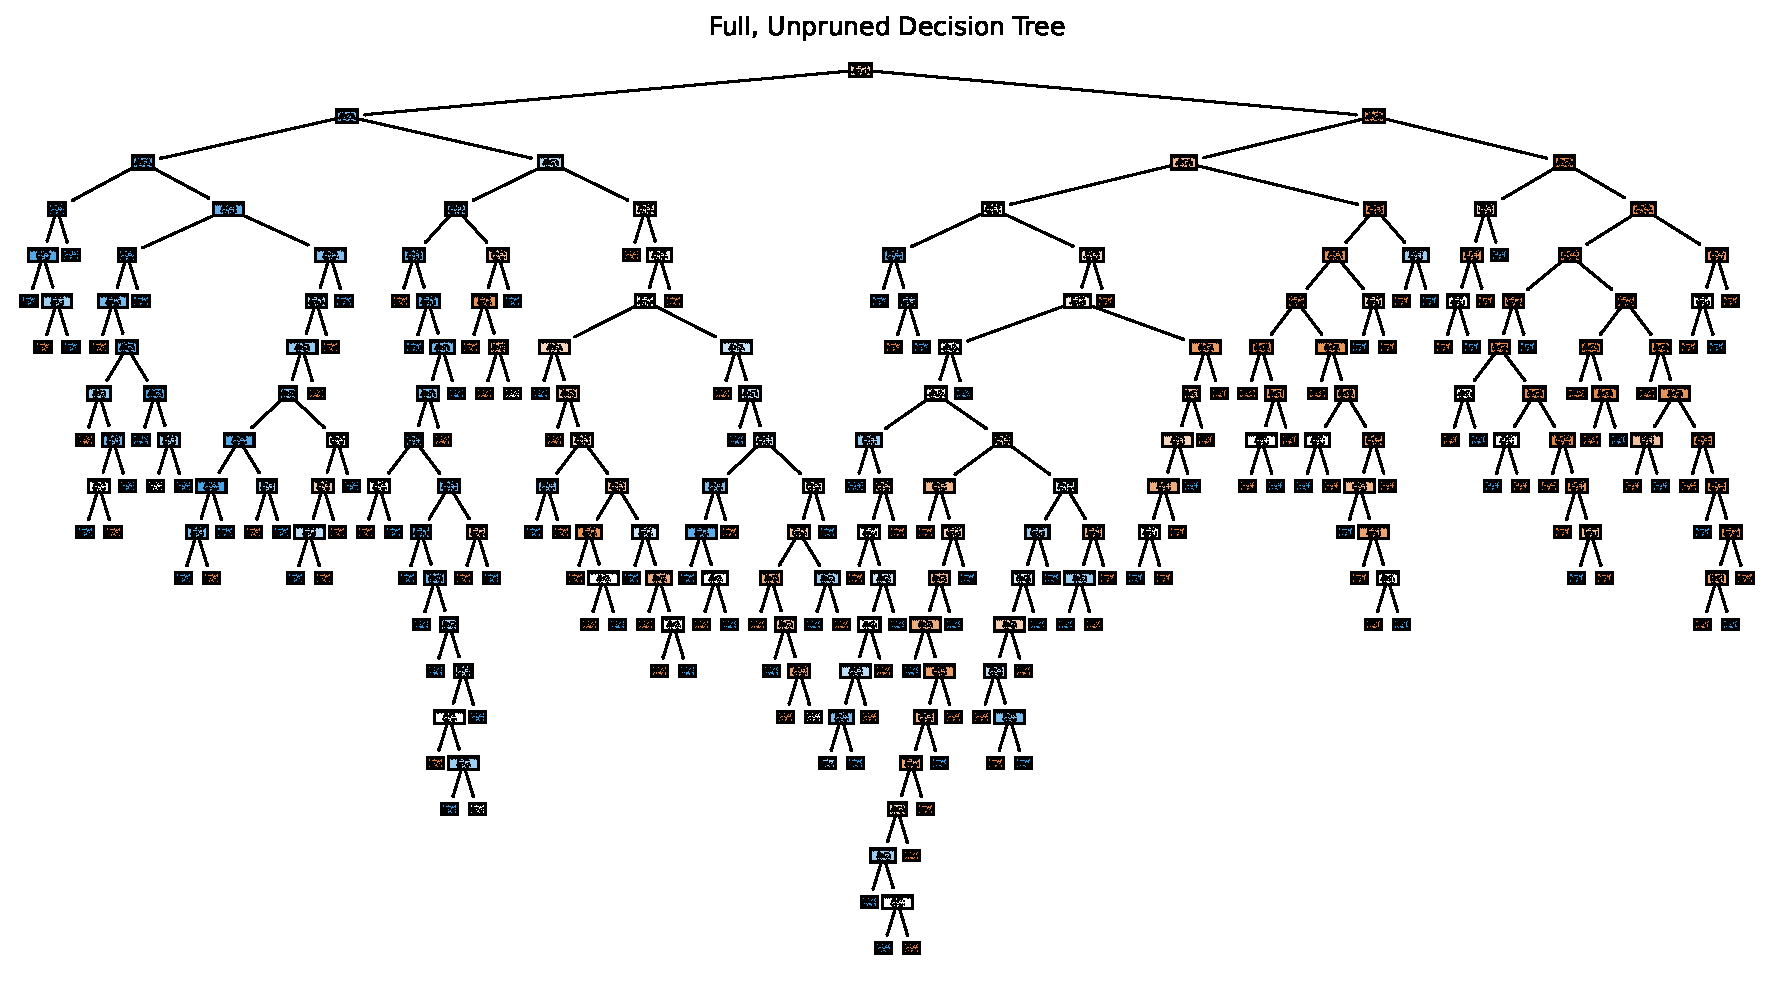
\includegraphics{Untitled-1_files/figure-pdf/cell-11-output-1.pdf}

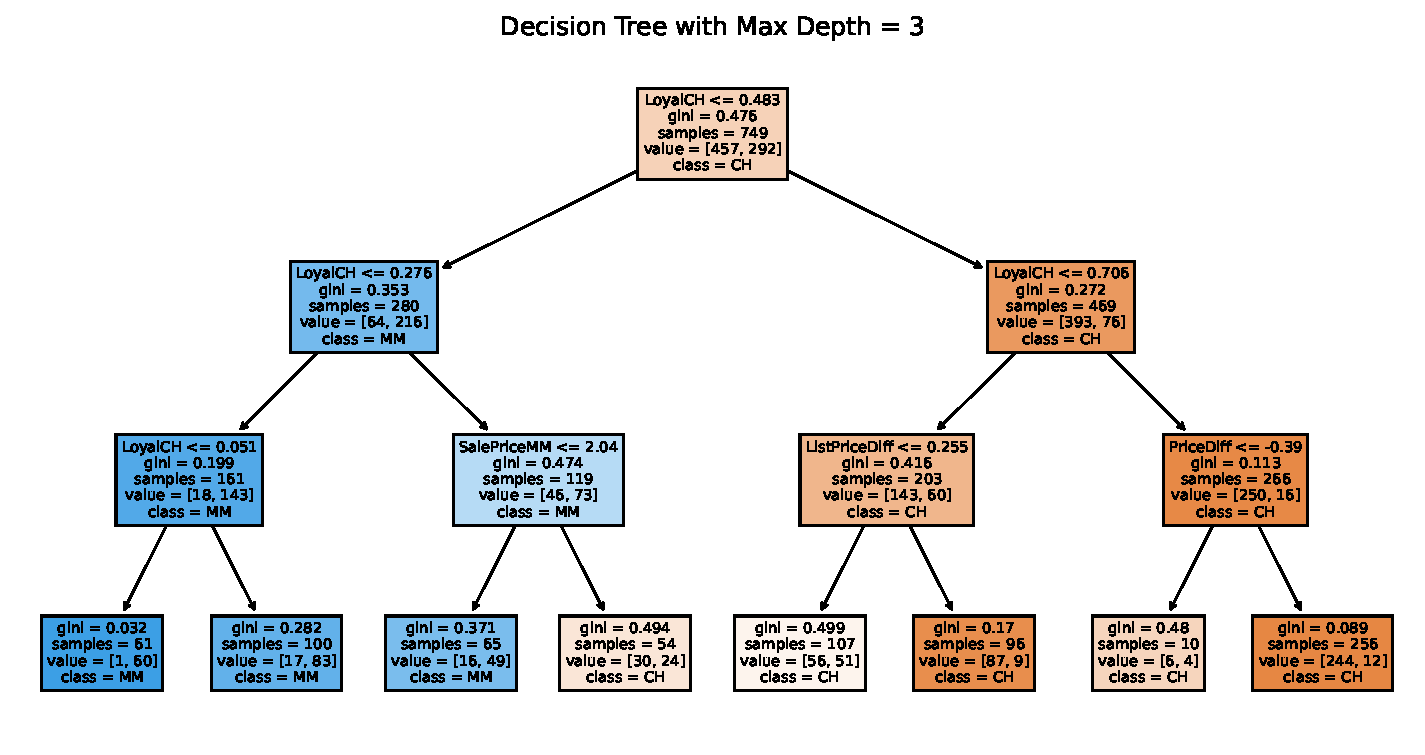
\includegraphics{Untitled-1_files/figure-pdf/cell-11-output-2.pdf}

\begin{verbatim}
Number of terminal nodes: 8
\end{verbatim}

Question 4d

\begin{Shaded}
\begin{Highlighting}[]
\CommentTok{\# make predictions on test set}
\NormalTok{y\_test\_pred }\OperatorTok{=}\NormalTok{ tree\_clf.predict(X\_test\_encoded)}

\CommentTok{\# generate the confusion matrix}
\NormalTok{conf\_matrix }\OperatorTok{=}\NormalTok{ confusion\_matrix(y\_test\_encoded, y\_test\_pred)}

\CommentTok{\# compute the test error rate}
\NormalTok{test\_accuracy }\OperatorTok{=}\NormalTok{ accuracy\_score(y\_test\_encoded, y\_test\_pred)}
\NormalTok{test\_error\_rate }\OperatorTok{=} \DecValTok{1} \OperatorTok{{-}}\NormalTok{ test\_accuracy}

\CommentTok{\# print results}
\BuiltInTok{print}\NormalTok{(}\StringTok{"Confusion Matrix:"}\NormalTok{)}
\BuiltInTok{print}\NormalTok{(conf\_matrix)}
\BuiltInTok{print}\NormalTok{(}\SpecialStringTok{f"Test Error Rate: }\SpecialCharTok{\{}\NormalTok{test\_error\_rate}\SpecialCharTok{:.4f\}}\SpecialStringTok{"}\NormalTok{)}
\end{Highlighting}
\end{Shaded}

\begin{verbatim}
Confusion Matrix:
[[160  36]
 [ 41  84]]
Test Error Rate: 0.2399
\end{verbatim}

Question 4e

\begin{Shaded}
\begin{Highlighting}[]
\CommentTok{\# fit an initial tree }
\NormalTok{tree\_clf }\OperatorTok{=}\NormalTok{ DecisionTreeClassifier(random\_state }\OperatorTok{=} \DecValTok{2}\NormalTok{)}
\NormalTok{tree\_clf.fit(X\_train\_encoded, y\_train\_encoded)}

\CommentTok{\# get the cost complexity pruning path}
\NormalTok{path }\OperatorTok{=}\NormalTok{ tree\_clf.cost\_complexity\_pruning\_path(X\_train\_encoded, y\_train\_encoded)}
\NormalTok{ccp\_alphas }\OperatorTok{=}\NormalTok{ path.ccp\_alphas  }

\CommentTok{\# perform 5{-}fold }
\NormalTok{cv\_errors }\OperatorTok{=}\NormalTok{ []}

\ControlFlowTok{for}\NormalTok{ alpha }\KeywordTok{in}\NormalTok{ ccp\_alphas:}
\NormalTok{    pruned\_tree }\OperatorTok{=}\NormalTok{ DecisionTreeClassifier(random\_state }\OperatorTok{=} \DecValTok{2}\NormalTok{, ccp\_alpha }\OperatorTok{=}\NormalTok{ alpha)}
\NormalTok{    scores }\OperatorTok{=}\NormalTok{ cross\_val\_score(pruned\_tree, X\_train\_encoded, y\_train\_encoded, }
\NormalTok{                             cv }\OperatorTok{=} \DecValTok{5}\NormalTok{, scoring }\OperatorTok{=} \StringTok{\textquotesingle{}accuracy\textquotesingle{}}\NormalTok{)}
\NormalTok{    cv\_errors.append(}\DecValTok{1} \OperatorTok{{-}}\NormalTok{ scores.mean())  }

\CommentTok{\# find the optimal alpha }
\NormalTok{optimal\_alpha }\OperatorTok{=}\NormalTok{ ccp\_alphas[np.argmin(cv\_errors)]}

\CommentTok{\# plot the graph}
\NormalTok{plt.figure(figsize }\OperatorTok{=}\NormalTok{ (}\DecValTok{8}\NormalTok{, }\DecValTok{5}\NormalTok{))}
\NormalTok{plt.plot(ccp\_alphas, cv\_errors, marker }\OperatorTok{=} \StringTok{\textquotesingle{}o\textquotesingle{}}\NormalTok{, linestyle }\OperatorTok{=} \StringTok{\textquotesingle{}{-}\textquotesingle{}}\NormalTok{)}
\NormalTok{plt.xlabel(}\StringTok{"Alpha (ccp\_alpha)"}\NormalTok{)}
\NormalTok{plt.ylabel(}\StringTok{"Cross{-}Validated Classification Error Rate"}\NormalTok{)}
\NormalTok{plt.title(}\StringTok{"Cost Complexity Pruning: Alpha vs. Classification Error"}\NormalTok{)}
\NormalTok{plt.axvline(x }\OperatorTok{=}\NormalTok{ optimal\_alpha, color }\OperatorTok{=} \StringTok{\textquotesingle{}r\textquotesingle{}}\NormalTok{, linestyle }\OperatorTok{=} \StringTok{\textquotesingle{}{-}{-}\textquotesingle{}}\NormalTok{, label }\OperatorTok{=} \SpecialStringTok{f\textquotesingle{}Optimal Alpha: }\SpecialCharTok{\{}\NormalTok{optimal\_alpha}\SpecialCharTok{:.4f\}}\SpecialStringTok{\textquotesingle{}}\NormalTok{)}
\NormalTok{plt.legend()}
\NormalTok{plt.show()}

\CommentTok{\# print results}
\BuiltInTok{print}\NormalTok{(}\SpecialStringTok{f"Optimal Alpha: }\SpecialCharTok{\{}\NormalTok{optimal\_alpha}\SpecialCharTok{:.4f\}}\SpecialStringTok{"}\NormalTok{)}
\end{Highlighting}
\end{Shaded}

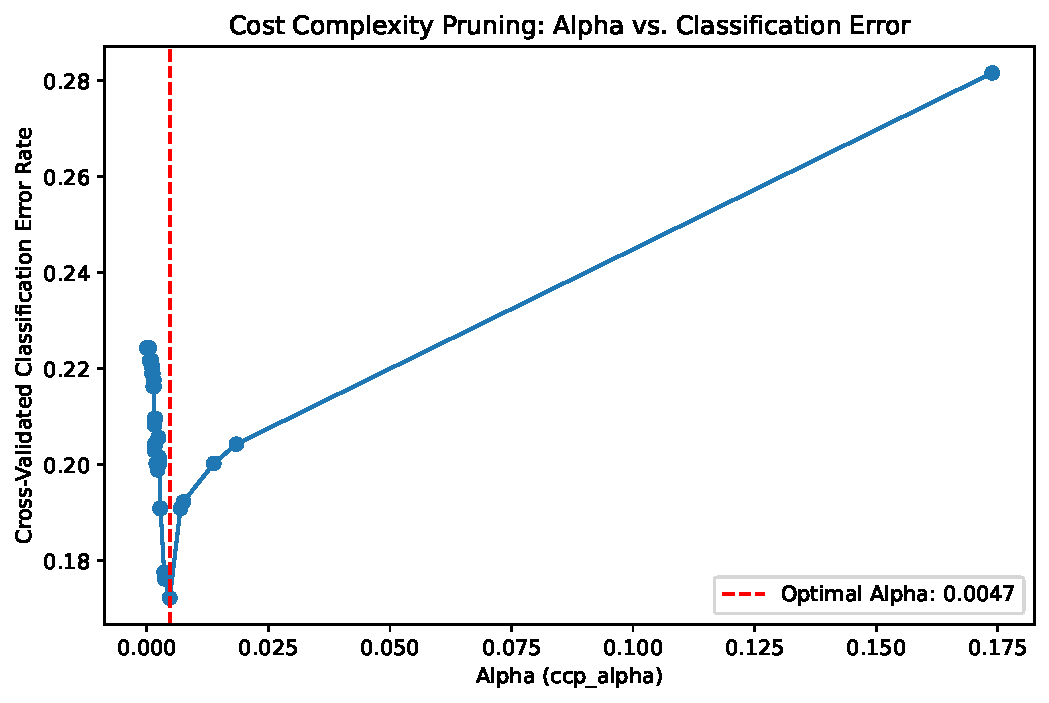
\includegraphics{Untitled-1_files/figure-pdf/cell-13-output-1.pdf}

\begin{verbatim}
Optimal Alpha: 0.0047
\end{verbatim}

Question 4f

\begin{Shaded}
\begin{Highlighting}[]
\CommentTok{\# find the number of terminal nodes for each alpha}
\NormalTok{tree\_sizes }\OperatorTok{=}\NormalTok{ []}

\ControlFlowTok{for}\NormalTok{ alpha }\KeywordTok{in}\NormalTok{ ccp\_alphas:}
\NormalTok{    pruned\_tree }\OperatorTok{=}\NormalTok{ DecisionTreeClassifier(random\_state }\OperatorTok{=} \DecValTok{2}\NormalTok{, ccp\_alpha }\OperatorTok{=}\NormalTok{ alpha)}
\NormalTok{    pruned\_tree.fit(X\_train\_encoded, y\_train\_encoded)}
\NormalTok{    tree\_sizes.append(pruned\_tree.tree\_.node\_count) }

\CommentTok{\# plot the graph}
\NormalTok{plt.figure(figsize }\OperatorTok{=}\NormalTok{ (}\DecValTok{8}\NormalTok{, }\DecValTok{5}\NormalTok{))}
\NormalTok{plt.plot(tree\_sizes, cv\_errors, marker }\OperatorTok{=} \StringTok{\textquotesingle{}o\textquotesingle{}}\NormalTok{, linestyle }\OperatorTok{=} \StringTok{\textquotesingle{}{-}\textquotesingle{}}\NormalTok{)}
\NormalTok{plt.xlabel(}\StringTok{"Tree Size (Number of Nodes)"}\NormalTok{)}
\NormalTok{plt.ylabel(}\StringTok{"Cross{-}Validated Classification Error Rate"}\NormalTok{)}
\NormalTok{plt.title(}\StringTok{"Tree Size vs. Classification Error Rate"}\NormalTok{)}
\NormalTok{plt.axvline(x }\OperatorTok{=}\NormalTok{ tree\_sizes[np.argmin(cv\_errors)], color }\OperatorTok{=} \StringTok{\textquotesingle{}r\textquotesingle{}}\NormalTok{, linestyle }\OperatorTok{=} \StringTok{\textquotesingle{}{-}{-}\textquotesingle{}}\NormalTok{, }
\NormalTok{            label }\OperatorTok{=} \SpecialStringTok{f\textquotesingle{}Optimal Tree Size: }\SpecialCharTok{\{}\NormalTok{tree\_sizes[np.argmin(cv\_errors)]}\SpecialCharTok{\}}\SpecialStringTok{\textquotesingle{}}\NormalTok{)}
\NormalTok{plt.legend()}
\NormalTok{plt.show()}

\CommentTok{\# print results}
\NormalTok{optimal\_tree\_size }\OperatorTok{=}\NormalTok{ tree\_sizes[np.argmin(cv\_errors)]}
\BuiltInTok{print}\NormalTok{(}\SpecialStringTok{f"Optimal Tree Size: }\SpecialCharTok{\{}\NormalTok{optimal\_tree\_size}\SpecialCharTok{\}}\SpecialStringTok{"}\NormalTok{)}
\end{Highlighting}
\end{Shaded}

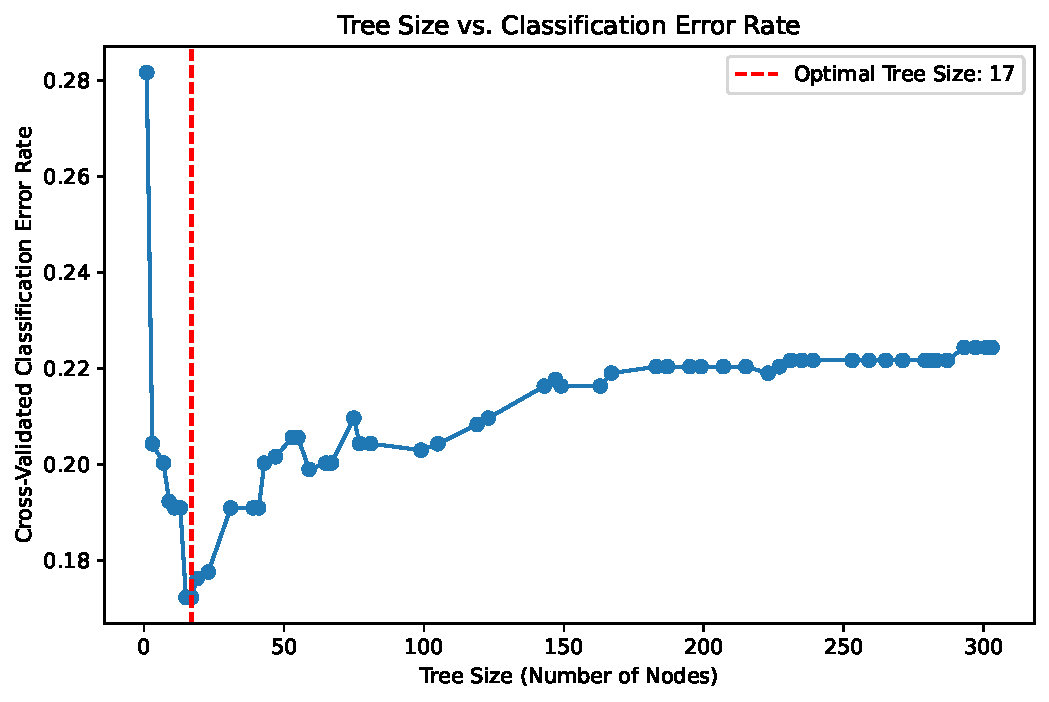
\includegraphics{Untitled-1_files/figure-pdf/cell-14-output-1.pdf}

\begin{verbatim}
Optimal Tree Size: 17
\end{verbatim}

Question 4g

\begin{Shaded}
\begin{Highlighting}[]
\CommentTok{\# fit the optimal pruned tree }
\NormalTok{optimal\_pruned\_tree }\OperatorTok{=}\NormalTok{ DecisionTreeClassifier(random\_state }\OperatorTok{=} \DecValTok{2}\NormalTok{, ccp\_alpha }\OperatorTok{=}\NormalTok{ optimal\_alpha)}
\NormalTok{optimal\_pruned\_tree.fit(X\_train\_encoded, y\_train\_encoded)}

\CommentTok{\# plot the graph}
\NormalTok{plt.figure(figsize }\OperatorTok{=}\NormalTok{ (}\DecValTok{12}\NormalTok{, }\DecValTok{6}\NormalTok{))}
\NormalTok{plot\_tree(optimal\_pruned\_tree, filled }\OperatorTok{=} \VariableTok{True}\NormalTok{, feature\_names }\OperatorTok{=}\NormalTok{ X\_train\_encoded.columns, }
\NormalTok{          class\_names }\OperatorTok{=}\NormalTok{ label\_encoder.classes\_)}
\NormalTok{plt.title(}\StringTok{"Optimal Pruned Decision Tree"}\NormalTok{)}
\NormalTok{plt.show()}
\end{Highlighting}
\end{Shaded}

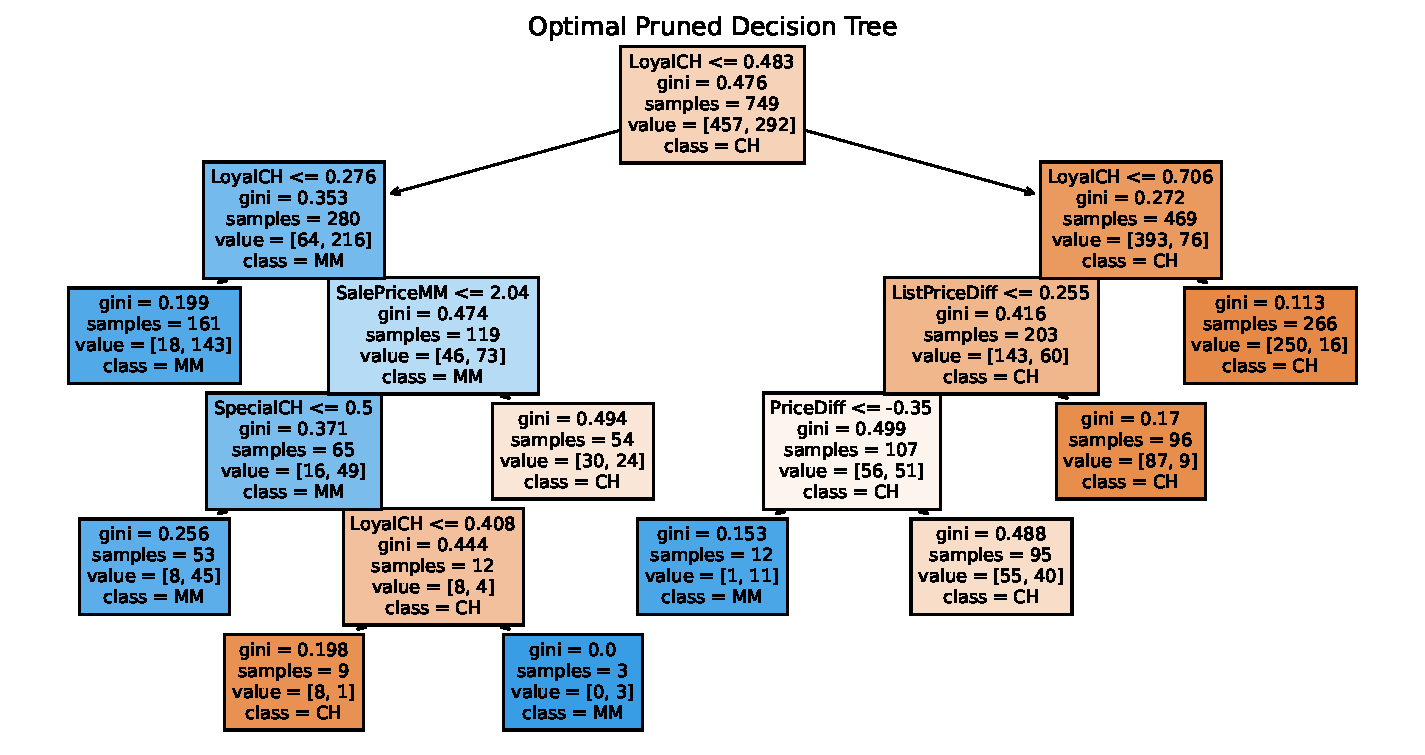
\includegraphics{Untitled-1_files/figure-pdf/cell-15-output-1.pdf}

Question 4h

\begin{Shaded}
\begin{Highlighting}[]
\CommentTok{\# find training error rate for the pruned tree}
\NormalTok{y\_train\_pred\_pruned }\OperatorTok{=}\NormalTok{ optimal\_pruned\_tree.predict(X\_train\_encoded)}
\NormalTok{train\_accuracy\_pruned }\OperatorTok{=}\NormalTok{ accuracy\_score(y\_train\_encoded, y\_train\_pred\_pruned)}
\NormalTok{train\_error\_rate\_pruned }\OperatorTok{=} \DecValTok{1} \OperatorTok{{-}}\NormalTok{ train\_accuracy\_pruned}

\CommentTok{\# print results}
\BuiltInTok{print}\NormalTok{(}\SpecialStringTok{f"Unpruned Tree Training Error Rate: }\SpecialCharTok{\{}\NormalTok{train\_error\_rate}\SpecialCharTok{:.4f\}}\SpecialStringTok{"}\NormalTok{)}
\BuiltInTok{print}\NormalTok{(}\SpecialStringTok{f"Pruned Tree Training Error Rate: }\SpecialCharTok{\{}\NormalTok{train\_error\_rate\_pruned}\SpecialCharTok{:.4f\}}\SpecialStringTok{"}\NormalTok{)}
\end{Highlighting}
\end{Shaded}

\begin{verbatim}
Unpruned Tree Training Error Rate: 0.0067
Pruned Tree Training Error Rate: 0.1562
\end{verbatim}

The unpruned tree has a training error of 0.67\%, while the pruned
tree's training error is 15.62\%. Pruning removes unnecessary branches,
making the tree simpler and better at handling new data. The unpruned
tree memorizes the training data, which gives it a very low training
error but likely a higher test error. The pruned tree has a higher
training error but is expected to perform better on new data because it
avoids overfitting.

Question 4i

\begin{Shaded}
\begin{Highlighting}[]
\CommentTok{\# find test error rate for the pruned tree}
\NormalTok{y\_test\_pred\_pruned }\OperatorTok{=}\NormalTok{ optimal\_pruned\_tree.predict(X\_test\_encoded)}
\NormalTok{test\_accuracy\_pruned }\OperatorTok{=}\NormalTok{ accuracy\_score(y\_test\_encoded, y\_test\_pred\_pruned)}
\NormalTok{test\_error\_rate\_pruned }\OperatorTok{=} \DecValTok{1} \OperatorTok{{-}}\NormalTok{ test\_accuracy\_pruned}

\CommentTok{\# print results}
\BuiltInTok{print}\NormalTok{(}\SpecialStringTok{f"Unpruned Tree Test Error Rate: }\SpecialCharTok{\{}\NormalTok{test\_error\_rate}\SpecialCharTok{:.4f\}}\SpecialStringTok{"}\NormalTok{)}
\BuiltInTok{print}\NormalTok{(}\SpecialStringTok{f"Pruned Tree Test Error Rate: }\SpecialCharTok{\{}\NormalTok{test\_error\_rate\_pruned}\SpecialCharTok{:.4f\}}\SpecialStringTok{"}\NormalTok{)}
\end{Highlighting}
\end{Shaded}

\begin{verbatim}
Unpruned Tree Test Error Rate: 0.2399
Pruned Tree Test Error Rate: 0.1963
\end{verbatim}

The unpruned tree's test error is 24.3\%, while the pruned tree's test
error is 19.63\%. Pruning removes unnecessary splits that fit noise in
the training data, helping the tree generalize better to new data. This
reduces test errors. The unpruned tree overfits, meaning it performs
well on training data but struggles with new data, leading to a higher
test error.




\end{document}
